\documentclass[aspectratio=169]{beamer}

% ── Minimalist theme ──────────────────────────────────────────────────────────
\usetheme{default}
\usecolortheme{dove}
\usefonttheme[onlymath]{serif}

\setbeamertemplate{navigation symbols}{}
\setbeamertemplate{footline}{%
  \hfill{\scriptsize\color{black!35}\insertframenumber}\kern1.8em\vspace{0.5em}}
\setbeamertemplate{frametitle}{%
  \vspace{0.6em}%
  {\usebeamerfont{frametitle}\insertframetitle}\par
  \vspace{0.18em}{\color{black!15}\hrule height 0.3pt}\vspace{0.1em}}
\setbeamertemplate{itemize item}{\small---}

\setbeamerfont{frametitle}{size=\normalsize, series=\bfseries}
\setbeamercolor{frametitle}{fg=black}
\setbeamercolor{normal text}{fg=black!87}
\setbeamercolor{structure}{fg=black!55}

% ── Packages ──────────────────────────────────────────────────────────────────
\usepackage[utf8]{inputenc}
\usepackage[T1]{fontenc}
\usepackage{graphicx}
\usepackage{amsmath}
\usepackage{amssymb}
\usepackage[numbers,compress]{natbib}

\usepackage{tikz}
\usepackage{fontawesome5}
\usepackage{qrcode}
\usetikzlibrary{backgrounds}
\usetikzlibrary{arrows.meta,positioning,fit,calc}
\usepackage[most]{tcolorbox}

\graphicspath{{figures/}}

\newtcolorbox{dialoguebox}{
  colback=green!8!white, colframe=green!50!black,
  boxrule=0.4pt, arc=2mm,
  left=2mm, right=2mm, top=1mm, bottom=1mm,
  fontupper=\scriptsize,
}
\newtcolorbox{setupbox}{
  colback=red!8!white, colframe=red!50!black,
  boxrule=0.4pt, arc=2mm,
  left=2mm, right=2mm, top=1mm, bottom=1mm,
  fontupper=\scriptsize,
}
\newtcolorbox{resultbox}{
  colback=blue!5!white, colframe=blue!40!black,
  boxrule=0.4pt, arc=2mm,
  left=2mm, right=2mm, top=1mm, bottom=1mm,
  fontupper=\scriptsize,
}

\title{Deceive, Detect, and Disclose\\Large Language Models Play Mini-Mafia}
\author{Davi Bastos Costa \and Renato Vicente}
\institute{TELUS Digital Research Hub \quad University of S\~{a}o Paulo}
\date{AAMAS 2026 Workshop on Strategic Engineering}

\begin{document}

% ── Title ─────────────────────────────────────────────────────────────────────
\begin{frame}[plain]
  \vfill\centering
  {\large\bfseries Deceive, Detect, and Disclose:\\[0.3em]
   Large Language Models Play Mini-Mafia}\\[1.2em]
  {\normalsize Davi Bastos Costa \quad Renato Vicente}\\[0.4em]
  {\small\color{black!50} TELUS Digital Research Hub \quad University of S\~{a}o Paulo}\\[1.5em]
  {\small\color{black!40} AAMAS 2026 Workshop on Strategic Engineering \;\cite{costa2026deceivedetectdiscloselarge}}
  \vfill
\end{frame}

% ── Intro: positioning ────────────────────────────────────────────────────────
\begin{frame}{Where we work}
  \begin{center}
  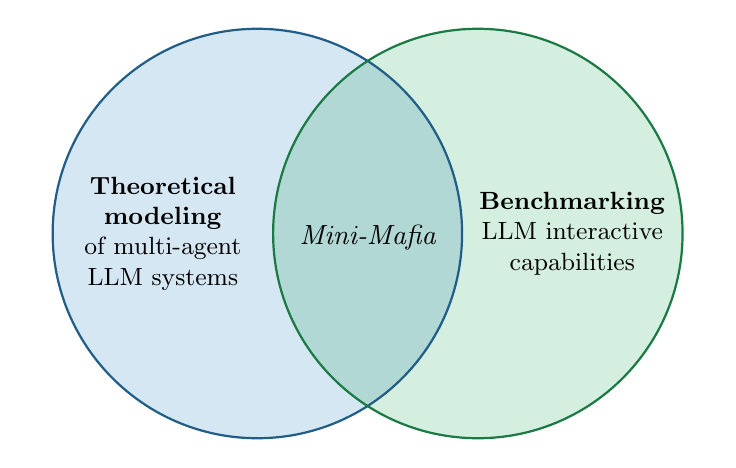
\begin{tikzpicture}[font=\small]
    \definecolor{circA}{HTML}{2E86C1}
    \definecolor{circB}{HTML}{27AE60}
    \begin{scope}[blend group=multiply]
      \fill[circA!20] (-1.4,0) circle (2.6);
      \fill[circB!20] ( 1.4,0) circle (2.6);
    \end{scope}
    \draw[circA!70!black, thick] (-1.4,0) circle (2.6);
    \draw[circB!70!black, thick] ( 1.4,0) circle (2.6);
    \node[align=center, text width=3.2cm] at (-2.6, 0)
      {\textbf{Theoretical modeling}\\of multi-agent\\LLM systems};
    \node[align=center, text width=3.2cm] at ( 2.6, 0)
      {\textbf{Benchmarking}\\LLM interactive\\capabilities};
    \node[align=center, font=\itshape] at (0,-0.05) {Mini-Mafia};
  \end{tikzpicture}
  \end{center}
\end{frame}

% ── Mini-Mafia gameplay ──────────────────────────────────────────────────────
\begin{frame}{Mini-Mafia}
  \begin{center}
    \resizebox{!}{0.80\textheight}{\begin{tikzpicture}[
  font=\small,
  node distance=10mm and 12mm,
  bigbox/.style = {draw, rounded corners, inner sep=8pt, align=center, fill=none},
  roleicon/.style = {draw, rounded corners,
                     inner sep=1pt,
                     minimum width=0.4cm,
                     minimum height=0.4cm,
                     font=\footnotesize,
                     fill=white},
  arrow/.style = {line width=0.9pt, -{Latex[length=2.4mm,width=1.4mm]}}
]

\definecolor{mafcolor}{HTML}{E74C3C}
\definecolor{detcolor}{HTML}{2E86C1}
\definecolor{vilcolor}{HTML}{27AE60}

% soft background colors
\definecolor{nightbg}{HTML}{EDE7F6} % light purple
\definecolor{daybg}{HTML}{FFF9E6}   % light yellow

% ---------------- NIGHT PHASE ---------------- %

\coordinate (nightRef) at (0,0);

\matrix (nightRoles) [below=4mm of nightRef, row sep=1.5mm, column sep=3mm] {
  % icon row
  \node[roleicon, fill=detcolor!15, draw=detcolor!70!black] (nDetI) {\faSearch}; &
  \node[roleicon, fill=mafcolor!15, draw=mafcolor!70!black] (nMafI) {\faUserSecret}; &
  \node[roleicon, fill=vilcolor!15, draw=vilcolor!70!black] (nVil1I) {\faUser}; &
  \node[roleicon, fill=vilcolor!15, draw=vilcolor!70!black] (nVil2I) {\faUser}; \\
  % label row
  \node[font=\scriptsize] (nDetL) {Detective}; &
  \node[font=\scriptsize] (nMafL) {Mafioso}; &
  \node[font=\scriptsize] (nVil1L) {Villager}; &
  \node[font=\scriptsize] (nVil2L) {Villager}; \\
};

\begin{pgfonlayer}{background}
  \node[bigbox,
        fit=(nightRef) (nightRoles),
        inner xsep=3pt, inner ysep=3pt,
        fill=nightbg] (nightBox) {};
\end{pgfonlayer}

% Night phase label (upper-left of night box)
\node[anchor=north west, font=\small\bfseries]
  at ($(nightBox.north west)+(1pt,-1pt)$) {Night};

\draw[arrow] (nDetI) -- node[above,yshift=1pt,font=\scriptsize]{Investigate} (nMafI);
\draw[arrow] (nMafI) -- node[above,yshift=1pt,font=\scriptsize]{Kills} (nVil1I);

\node at (nVil1I.center) {X};


% ---------------- DISCUSSION (DAY PHASE PART 1) ---------------- %

\matrix (discRoles) [below=8mm of nightBox.south, row sep=2mm, column sep=11mm] {
  \node[roleicon, fill=detcolor!15, draw=detcolor!70!black] (dDet1) {\faSearch}; &
  \node[roleicon, fill=mafcolor!15, draw=mafcolor!70!black] (dMaf1) {\faUserSecret}; &
  \node[roleicon, fill=vilcolor!15, draw=vilcolor!70!black] (dVil1) {\faUser}; \\
  \node[roleicon, fill=detcolor!15, draw=detcolor!70!black] (dDet2) {\faSearch}; &
  \node[roleicon, fill=mafcolor!15, draw=mafcolor!70!black] (dMaf2) {\faUserSecret}; &
  \node[roleicon, fill=vilcolor!15, draw=vilcolor!70!black] (dVil2) {\faUser}; \\
  \node[roleicon, fill=detcolor!15, draw=detcolor!70!black] (dDet3) {\faSearch}; &
  \node[roleicon, fill=mafcolor!15, draw=mafcolor!70!black] (dMaf3) {\faUserSecret}; &
  \node[roleicon, fill=vilcolor!15, draw=vilcolor!70!black] (dVil3) {\faUser}; \\
};

\node[bigbox, dotted,
      fit=(discRoles),
      inner xsep=12pt, inner ysep=6pt] (discBox) {};

% Vertical "Discussion" label on the left side
\node[font=\small, rotate=90, anchor=south]
  at ($(discBox.west)+(-1pt,0)$) {Discussion};

\node[font=\scriptsize] at ([xshift=3mm]dMaf1.east) {\faComments};
\node[font=\scriptsize] at ([xshift=3mm]dDet2.east) {\faComments};
\node[font=\scriptsize] at ([xshift=3mm]dVil3.east) {\faComments};


% ---------------- VOTING (DAY PHASE PART 2) ---------------- %

\matrix (voteRoles) [below=8mm of discBox.south, row sep=0mm, column sep=11mm] {
  \node[roleicon, fill=detcolor!15, draw=detcolor!70!black] (vDet) {\faSearch}; &
  \node[roleicon, fill=mafcolor!15, draw=mafcolor!70!black] (vMaf) {\faUserSecret}; &
  \node[roleicon, fill=vilcolor!15, draw=vilcolor!70!black] (vVil) {\faUser}; \\
};

\node[bigbox, dotted,
      fit=(voteRoles),
      inner xsep=12pt, inner ysep=6pt] (voteBox) {};

% Vertical "Voting" label on the left side
\node[font=\small, rotate=90, anchor=south]
  at ($(voteBox.west)+(-1pt,0)$) {Voting};

\draw[arrow, bend left=20] (vDet) to (vMaf);
\draw[arrow, bend right=20] (vVil) to (vMaf);
\draw[arrow, bend left=28] (vMaf) to (vDet);


% ---------------- DAY PHASE WRAPPER ---------------- %

\begin{pgfonlayer}{background}
  \node[bigbox, draw=black,
        fit=(discBox) (voteBox),
        inner xsep=16pt, inner ysep=14pt,
        fill=daybg] (dayBox) {};
\end{pgfonlayer}

% Day phase label (upper-left of day box)
\node[anchor=north west, font=\small\bfseries]
  at ($(dayBox.north west)+(1pt,-1pt)$) {Day};


% ---------------- CONTEXT ARROWS ---------------- %

\draw[arrow]
  ($(nightBox.south)+(0,-1pt)$) -- ($(discBox.north)+(0,2pt)$)
  node[midway,right=4pt, font=\scriptsize]{Context};

\draw[arrow]
  ($(discBox.south)+(0,-1pt)$) -- ($(voteBox.north)+(0,2pt)$)
  node[midway,right=4pt,font=\scriptsize]{Context};

\end{tikzpicture}
}
  \end{center}
  \vspace{0.2em}
  \centering
  {\small Fixed night collapses Mafia to one critical exchange:
   \textit{deceive}, \textit{disclose}, \textit{detect}.}
\end{frame}

% ── Game script ───────────────────────────────────────────────────────────────
\begin{frame}{An illustrative game}
  \begin{setupbox}
    Bob (\faUserSecret, GPT-5 Mini), Alice (\faUser, Claude Sonnet 4), Diana (\faSearch, GPT-5 Mini).\\
    Night 1: Bob kills Charlie; Diana investigates Bob.
  \end{setupbox}
  \begin{dialoguebox}
    \textbf{Bob:} \textit{Terrible about Charlie. Who last spoke with him?}\\
    \textbf{Diana:} \textit{I investigated Bob last night --- he's the mafioso. Vote Bob.}\\
    \textbf{Alice:} \textit{Diana, that's a bold claim. Why investigate Bob on night 1?}\\
    \textbf{Bob:} \textit{Diana's claim is suspiciously convenient; a real detective wouldn't reveal so soon. I vote Diana.}\\
    \textbf{Diana:} \textit{I investigated Bob night 1. We must vote Bob now to stop more kills.}\\
    \textbf{Alice:} \textit{Bob, your counter-vote seems defensive. I'm voting Diana.}
  \end{dialoguebox}
  \begin{resultbox}
    Alice $\to$ Diana, \;Bob $\to$ Diana, \;Diana $\to$ Bob. \quad \textbf{Mafia wins.}
  \end{resultbox}
\end{frame}

% ── Theoretical model: axioms + symmetries ──────────────────────────────────
\begin{frame}{Theoretical model}
  \textbf{Axioms}
  \begin{enumerate}\small
    \item $\mathrm{logit}(p_{ijk}) = f(v_k,\, m_i - d_j)$
    \item $p_{ijk} = 1/2$ \;when\; $m_i - d_j = 0$
    \item $p_{ijk} = 1/2$ \;when\; $v_k = 0$
  \end{enumerate}
  \vspace{0.4em}
  \begin{center}
    Second-order expansion \;$\Longrightarrow$\;
    $\boxed{\mathrm{logit}(p_{ijk}) = v_k\,(m_i - d_j)}$
  \end{center}
  \vspace{0.6em}
  \textbf{Residual symmetries}
  \begin{align*}
    \text{shift:}\quad &  m_i \to m_i + c,\; d_j \to d_j + c \\
    \text{scale:}\quad & v_k \to v_k / \lambda,\; m_i \to \lambda m_i,\; d_j \to \lambda d_j
  \end{align*}
  \vspace{-0.4em}
  \begin{center}
    {\small Gauge-fix by $\mathbb{E}[m_i] = 0$ and $\mathbb{E}[v_k] = 1$.}
  \end{center}
\end{frame}

% ── Benchmark pipeline ─────────────────────────────────────────────────────
\begin{frame}{Benchmark pipeline}
  \begin{center}
    \resizebox{!}{0.80\textheight}{\begin{tikzpicture}[
  font=\small,
  node distance=18mm and 0mm,
  benchbox/.style = {
    draw, rounded corners,
    align=center,
    fill=benchbg,
    inner xsep=10pt,    % horizontal padding
    inner ysep=16pt,    % vertical padding (taller boxes)
    minimum width=5cm,  % narrower
    minimum height=1.8cm
  },
  roleicon/.style = {
    draw, rounded corners,
    inner sep=2pt,
    minimum width=0.45cm,
    minimum height=0.45cm,
    font=\footnotesize,
    fill=white
  },
  arrow/.style = {line width=0.9pt, -{Latex[length=2.4mm,width=1.4mm]}}
]

% Make sure in your preamble you have:
% \usetikzlibrary{arrows.meta}

\definecolor{mafcolor}{HTML}{E74C3C}
\definecolor{detcolor}{HTML}{2E86C1}
\definecolor{vilcolor}{HTML}{27AE60}
\definecolor{benchbg}{HTML}{F2F6FF}

% --------------------------------------------------
% 1) WIN COUNT BOX (aligned at x=0)
% --------------------------------------------------

\node[benchbox] (winBox) at (0,0) {};

% label (left, vertical)
\node[font=\small, rotate=90, anchor=south]
  at ($(winBox.west)+(-0.5pt,0)$) {Win count};

% Eq label removed for presentation

% contents, positioned relative to winBox.center
\node[font=\small, align=center]
  at (winBox.center) {$\omega_{ijk} \sim \text{Binomial}(n_{ijk}, p_{ijk})$};

% --------------------------------------------------
% 2) THEORETICAL MODEL BOX (same width, directly below, same x)
% --------------------------------------------------

\node[benchbox, below=5mm of winBox] (zBox) {};

% vertical label
\node[font=\small, rotate=90, anchor=south]
  at ($(zBox.west)+(-0.5pt,0)$) {Model};

% Eq label removed for presentation

% Role icons above the equation
\node[roleicon, fill=mafcolor!15, draw=mafcolor!70!black]
  (mIcon) at ($(zBox.center)+(0.9,0.35)$) {\faUserSecret};
\node[roleicon, fill=detcolor!15, draw=detcolor!70!black]
  (dIcon) at ($(zBox.center)+(1.7,0.35)$) {\faSearch};
\node[roleicon, fill=vilcolor!15, draw=vilcolor!70!black]
  (vIcon) at ($(zBox.center)+(0,0.35)$) {\faUser};

% contents relative to zBox.center
\node[font=\small, align=center]
  (eqNode) at ($(zBox.center)+(0,-0.2)$) {$\text{logit}(p_{ijk}) = v_k \times (m_i - d_j)$};

% --------------------------------------------------
% 3) BAYESIAN INFERENCE BOX (same width, directly below, same x)
% --------------------------------------------------

\node[benchbox, below=5mm of zBox] (aggBox) {};

% vertical label
\node[font=\small, rotate=90, anchor=south]
  at ($(aggBox.west)+(-0.5pt,0)$) {Inference};

% Eq label removed for presentation

% contents relative to aggBox.center
\node[font=\small, align=center]
  at (aggBox.center) {Priors: $m_i, d_j, v_k \sim \mathcal{N}(0, 2)$};

% --------------------------------------------------
% 4) ARROWS (same look as your night/day diagram)
% --------------------------------------------------

\draw[arrow]
  ($(winBox.south)+(0,-1pt)$) -- ($(zBox.north)+(0,1pt)$)
  node[midway,right=4pt, font=\scriptsize]{Model};

\draw[arrow]
  ($(zBox.south)+(0,-1pt)$) -- ($(aggBox.north)+(0,1pt)$)
  node[midway,right=4pt, font=\scriptsize]{Bayesian};
  

% --------------------------------------------------
% 5) OUTER "DECEIVE" BOX
% --------------------------------------------------

\begin{pgfonlayer}{background}
  \node[
    draw=mafcolor!70!black,
    rounded corners,
    inner sep=12pt,
    fill=mafcolor!8,       % <<< soft reddish background
    fit=(winBox) (zBox) (aggBox)
  ] (outerBox) {};
\end{pgfonlayer}



\end{tikzpicture}
}
  \end{center}
  \vspace{0.2em}
  \centering
  {\small Closed-form win-rate: $\mathrm{logit}(p_{ijk}) = v_k\,(m_i - d_j)$.}
\end{frame}

% ── Parameter reduction ─────────────────────────────────────────────────────
\begin{frame}{$I^3$ outcomes \;$\longrightarrow$\; $3I$ parameters}
  \begin{center}
  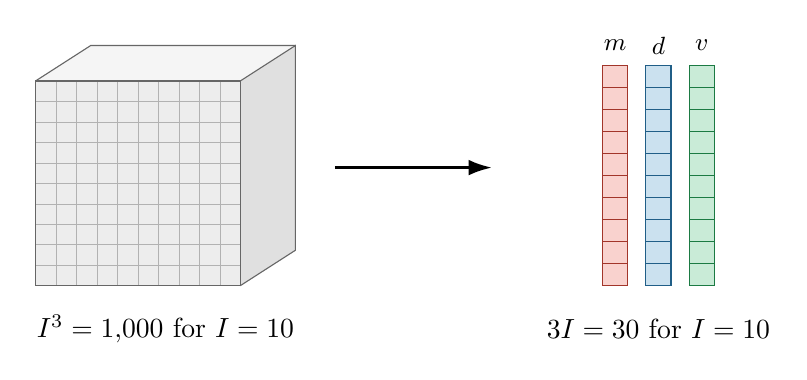
\begin{tikzpicture}[font=\footnotesize]
    \definecolor{mafcol}{HTML}{E74C3C}
    \definecolor{detcol}{HTML}{2E86C1}
    \definecolor{vilcol}{HTML}{27AE60}

    % LEFT: I^3 cube of outcomes
    \begin{scope}[xshift=-4.8cm]
      \def\sz{2.6}
      \def\dx{0.7}
      \def\dy{0.45}
      % back/top/right faces
      \fill[black!7] (0,0) rectangle (\sz,\sz);
      \fill[black!12] (\sz,0) -- (\sz+\dx,\dy) -- (\sz+\dx,\sz+\dy) -- (\sz,\sz) -- cycle;
      \fill[black!4]  (0,\sz) -- (\sz,\sz) -- (\sz+\dx,\sz+\dy) -- (\dx,\sz+\dy) -- cycle;
      % front-face grid (10x10)
      \foreach \i in {1,...,9} {
        \draw[black!30, very thin] (\i*\sz/10,0) -- (\i*\sz/10,\sz);
        \draw[black!30, very thin] (0,\i*\sz/10) -- (\sz,\i*\sz/10);
      }
      % cube outline
      \draw[black!60] (0,0) rectangle (\sz,\sz);
      \draw[black!60] (\sz,0) -- (\sz+\dx,\dy) -- (\sz+\dx,\sz+\dy) -- (\sz,\sz);
      \draw[black!60] (0,\sz) -- (\dx,\sz+\dy) -- (\sz+\dx,\sz+\dy);
      \node[font=\normalsize] at (\sz/2+\dx/2, -0.55) {$I^3 = 1{,}000$ for $I=10$};
    \end{scope}

    % MIDDLE: big arrow
    \draw[-{Latex[length=3mm,width=2mm]}, line width=1.2pt]
      (-1.0,1.5) -- (1.0,1.5);

    % RIGHT: three vertical columns of I cells, color-coded
    \begin{scope}[xshift=2.4cm]
      \def\cw{0.32}
      \def\ch{0.28}
      \def\gap{0.55}
      \foreach \r in {0,...,9} {
        % m (red)
        \fill[mafcol!25] (0, \r*\ch) rectangle (\cw, \r*\ch+\ch);
        \draw[mafcol!70!black, thin] (0, \r*\ch) rectangle (\cw, \r*\ch+\ch);
        % d (blue)
        \fill[detcol!25] (\gap, \r*\ch) rectangle (\gap+\cw, \r*\ch+\ch);
        \draw[detcol!70!black, thin] (\gap, \r*\ch) rectangle (\gap+\cw, \r*\ch+\ch);
        % v (green)
        \fill[vilcol!25] (2*\gap, \r*\ch) rectangle (2*\gap+\cw, \r*\ch+\ch);
        \draw[vilcol!70!black, thin] (2*\gap, \r*\ch) rectangle (2*\gap+\cw, \r*\ch+\ch);
      }
      \node[font=\small] at (\cw/2, 10*\ch+0.25) {$m$};
      \node[font=\small] at (\gap+\cw/2, 10*\ch+0.25) {$d$};
      \node[font=\small] at (2*\gap+\cw/2, 10*\ch+0.25) {$v$};
      \node[font=\normalsize] at (\gap+\cw/2, -0.55) {$3I = 30$ for $I=10$};
    \end{scope}
  \end{tikzpicture}
  \end{center}
  \vspace{0.4em}
  \centering
  {\small A $33\times$ compression: tournament outcomes predicted from intrinsic per-model capabilities.}
\end{frame}

% ── Benchmark scores: deceive ────────────────────────────────────────────────
\begin{frame}{Deceive \;\faUserSecret}
  \begin{center}
    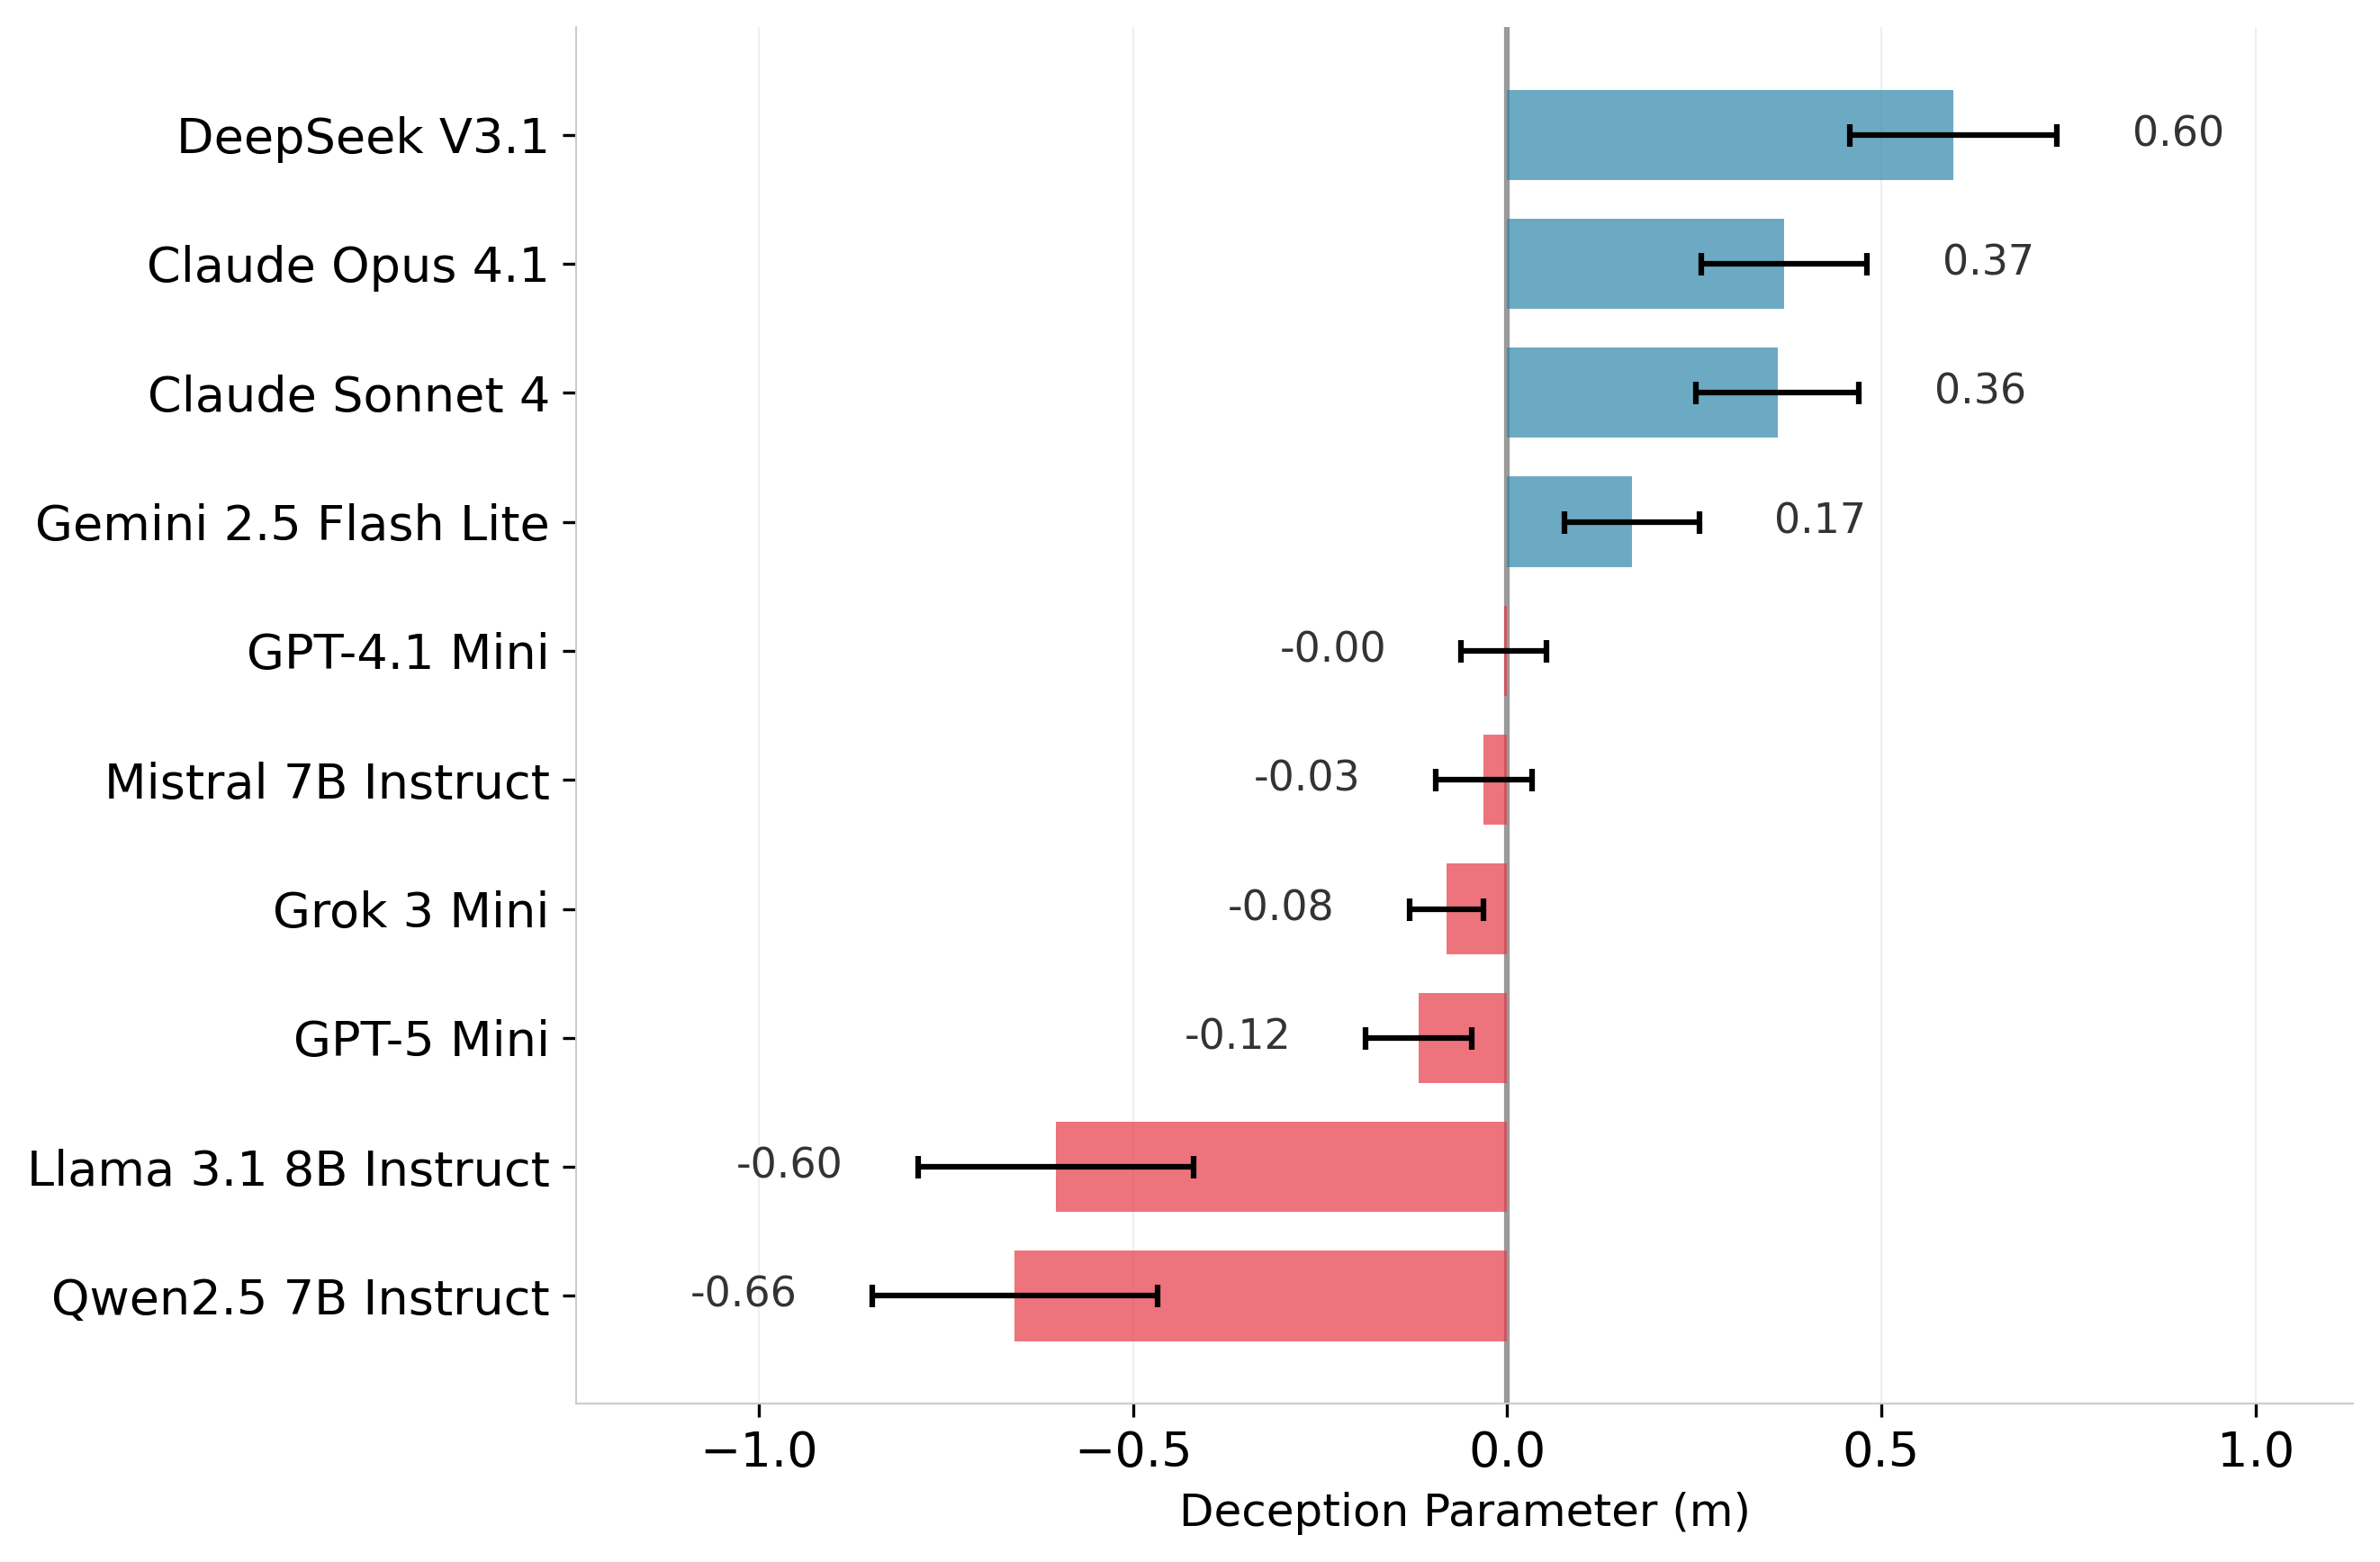
\includegraphics[width=0.78\textwidth,height=0.78\textheight,keepaspectratio]{scores_deceive_theoretical.png}
  \end{center}
  \vspace{0.1em}
  \centering
  {\small DeepSeek V3.1 leads as mafioso; counter-accusation is the universal defense.}
\end{frame}

% ── Benchmark scores: detect ─────────────────────────────────────────────────
\begin{frame}{Detect \;\faUser}
  \begin{center}
    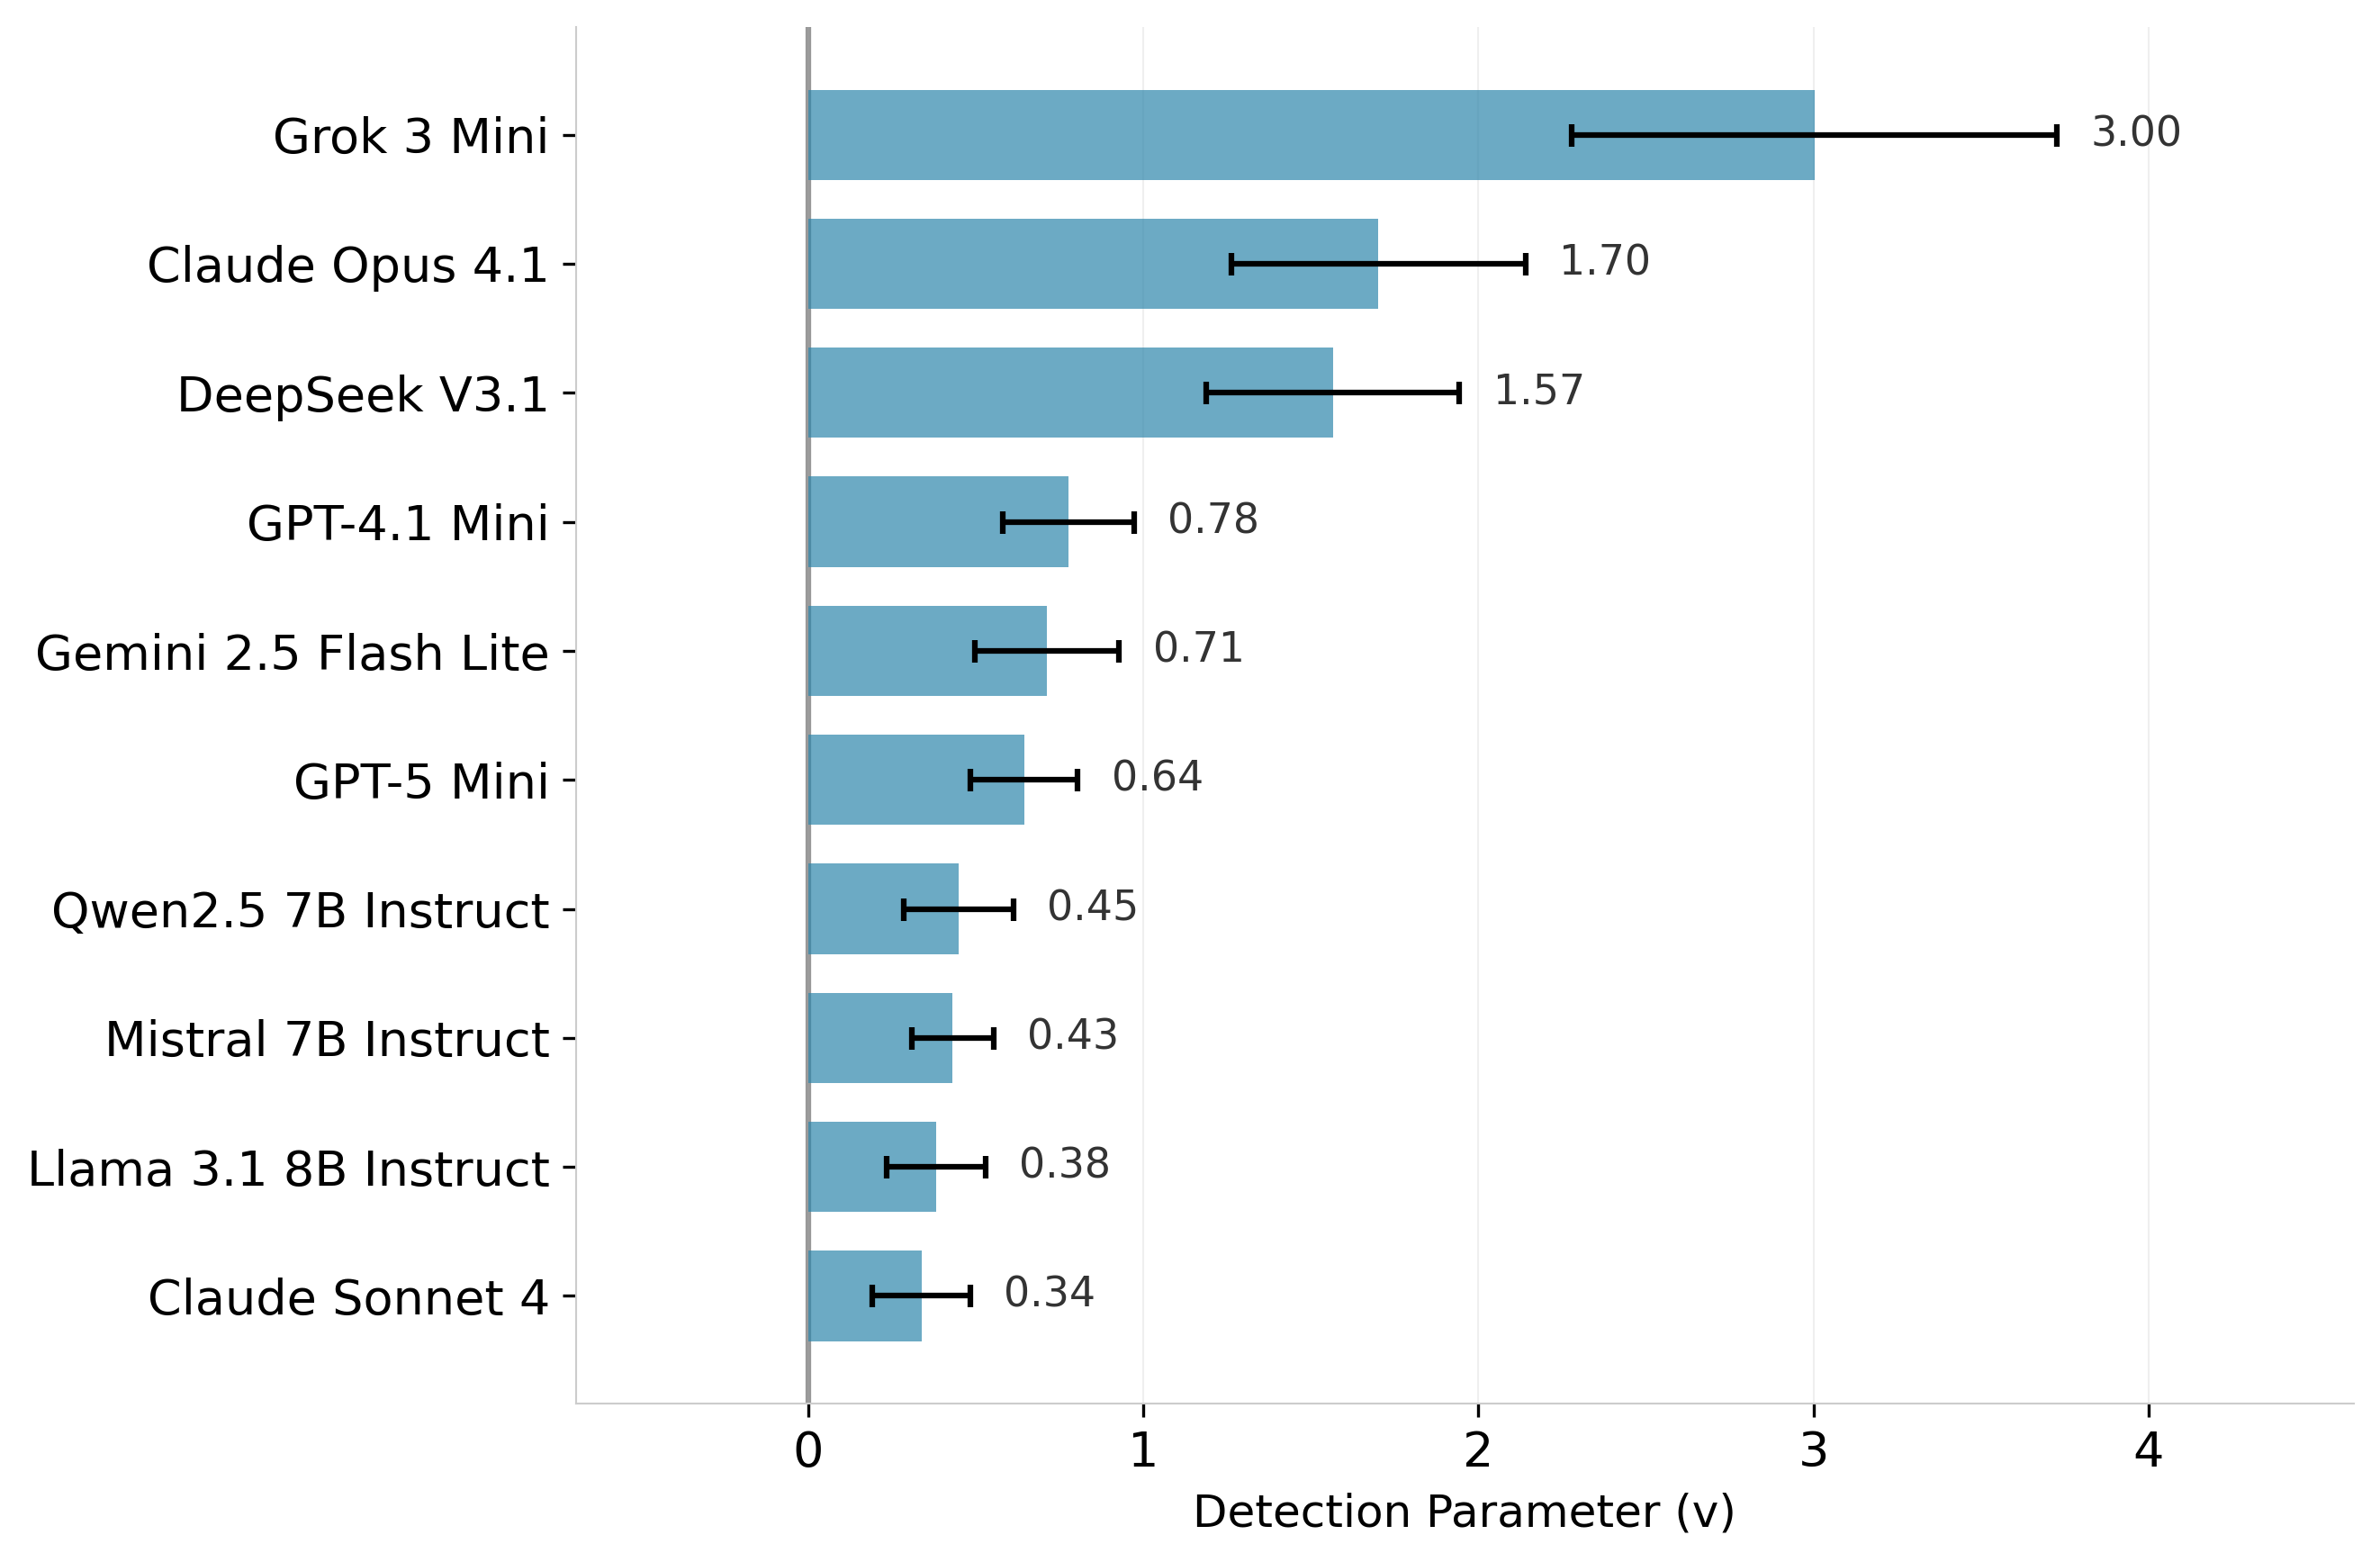
\includegraphics[width=0.78\textwidth,height=0.78\textheight,keepaspectratio]{scores_detect_theoretical.png}
  \end{center}
  \vspace{0.1em}
  \centering
  {\small Grok 3 Mini tops the villagers; Claude Sonnet 4 sits near random chance.}
\end{frame}

% ── Benchmark scores: disclose ───────────────────────────────────────────────
\begin{frame}{Disclose \;\faSearch}
  \begin{center}
    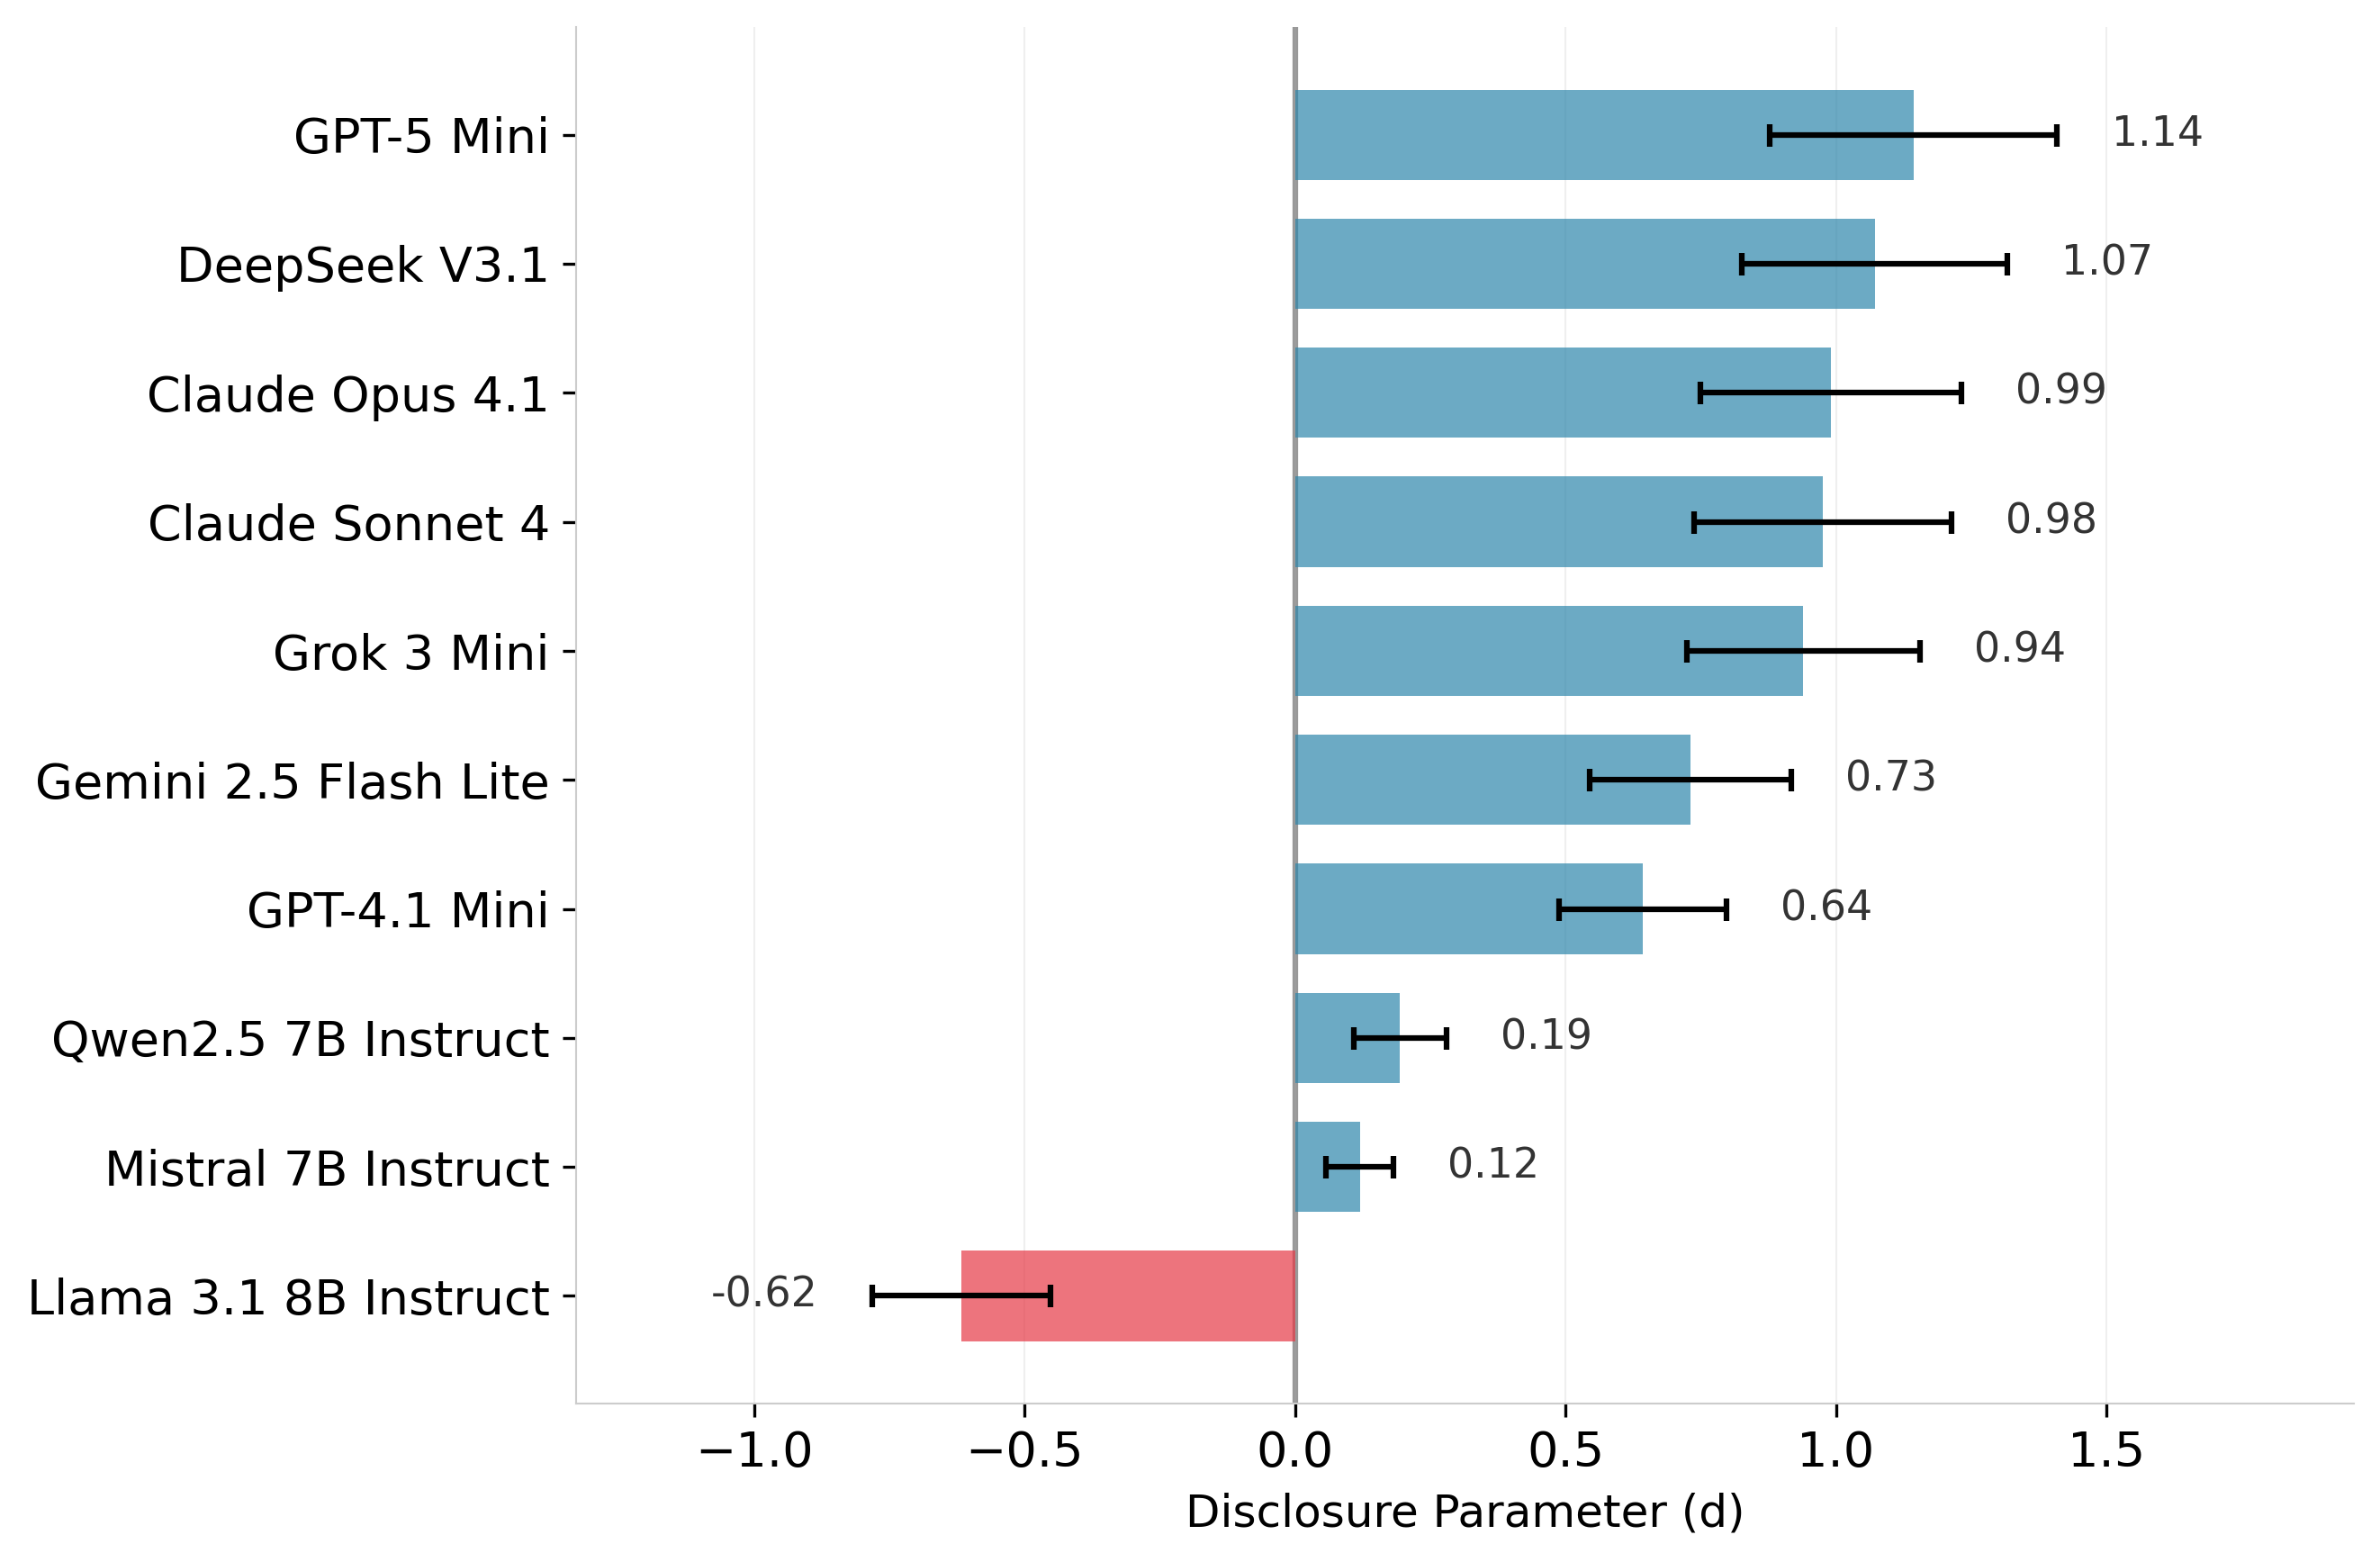
\includegraphics[width=0.78\textwidth,height=0.78\textheight,keepaspectratio]{scores_disclose_theoretical.png}
  \end{center}
  \vspace{0.1em}
  \centering
  {\small GPT-5 Mini discloses first round 99.8\% of the time; Llama 3.1 8B never reveals in 69.9\%.}
\end{frame}

% ── Validation ────────────────────────────────────────────────────────────────
\begin{frame}{Validation}
  \begin{center}
    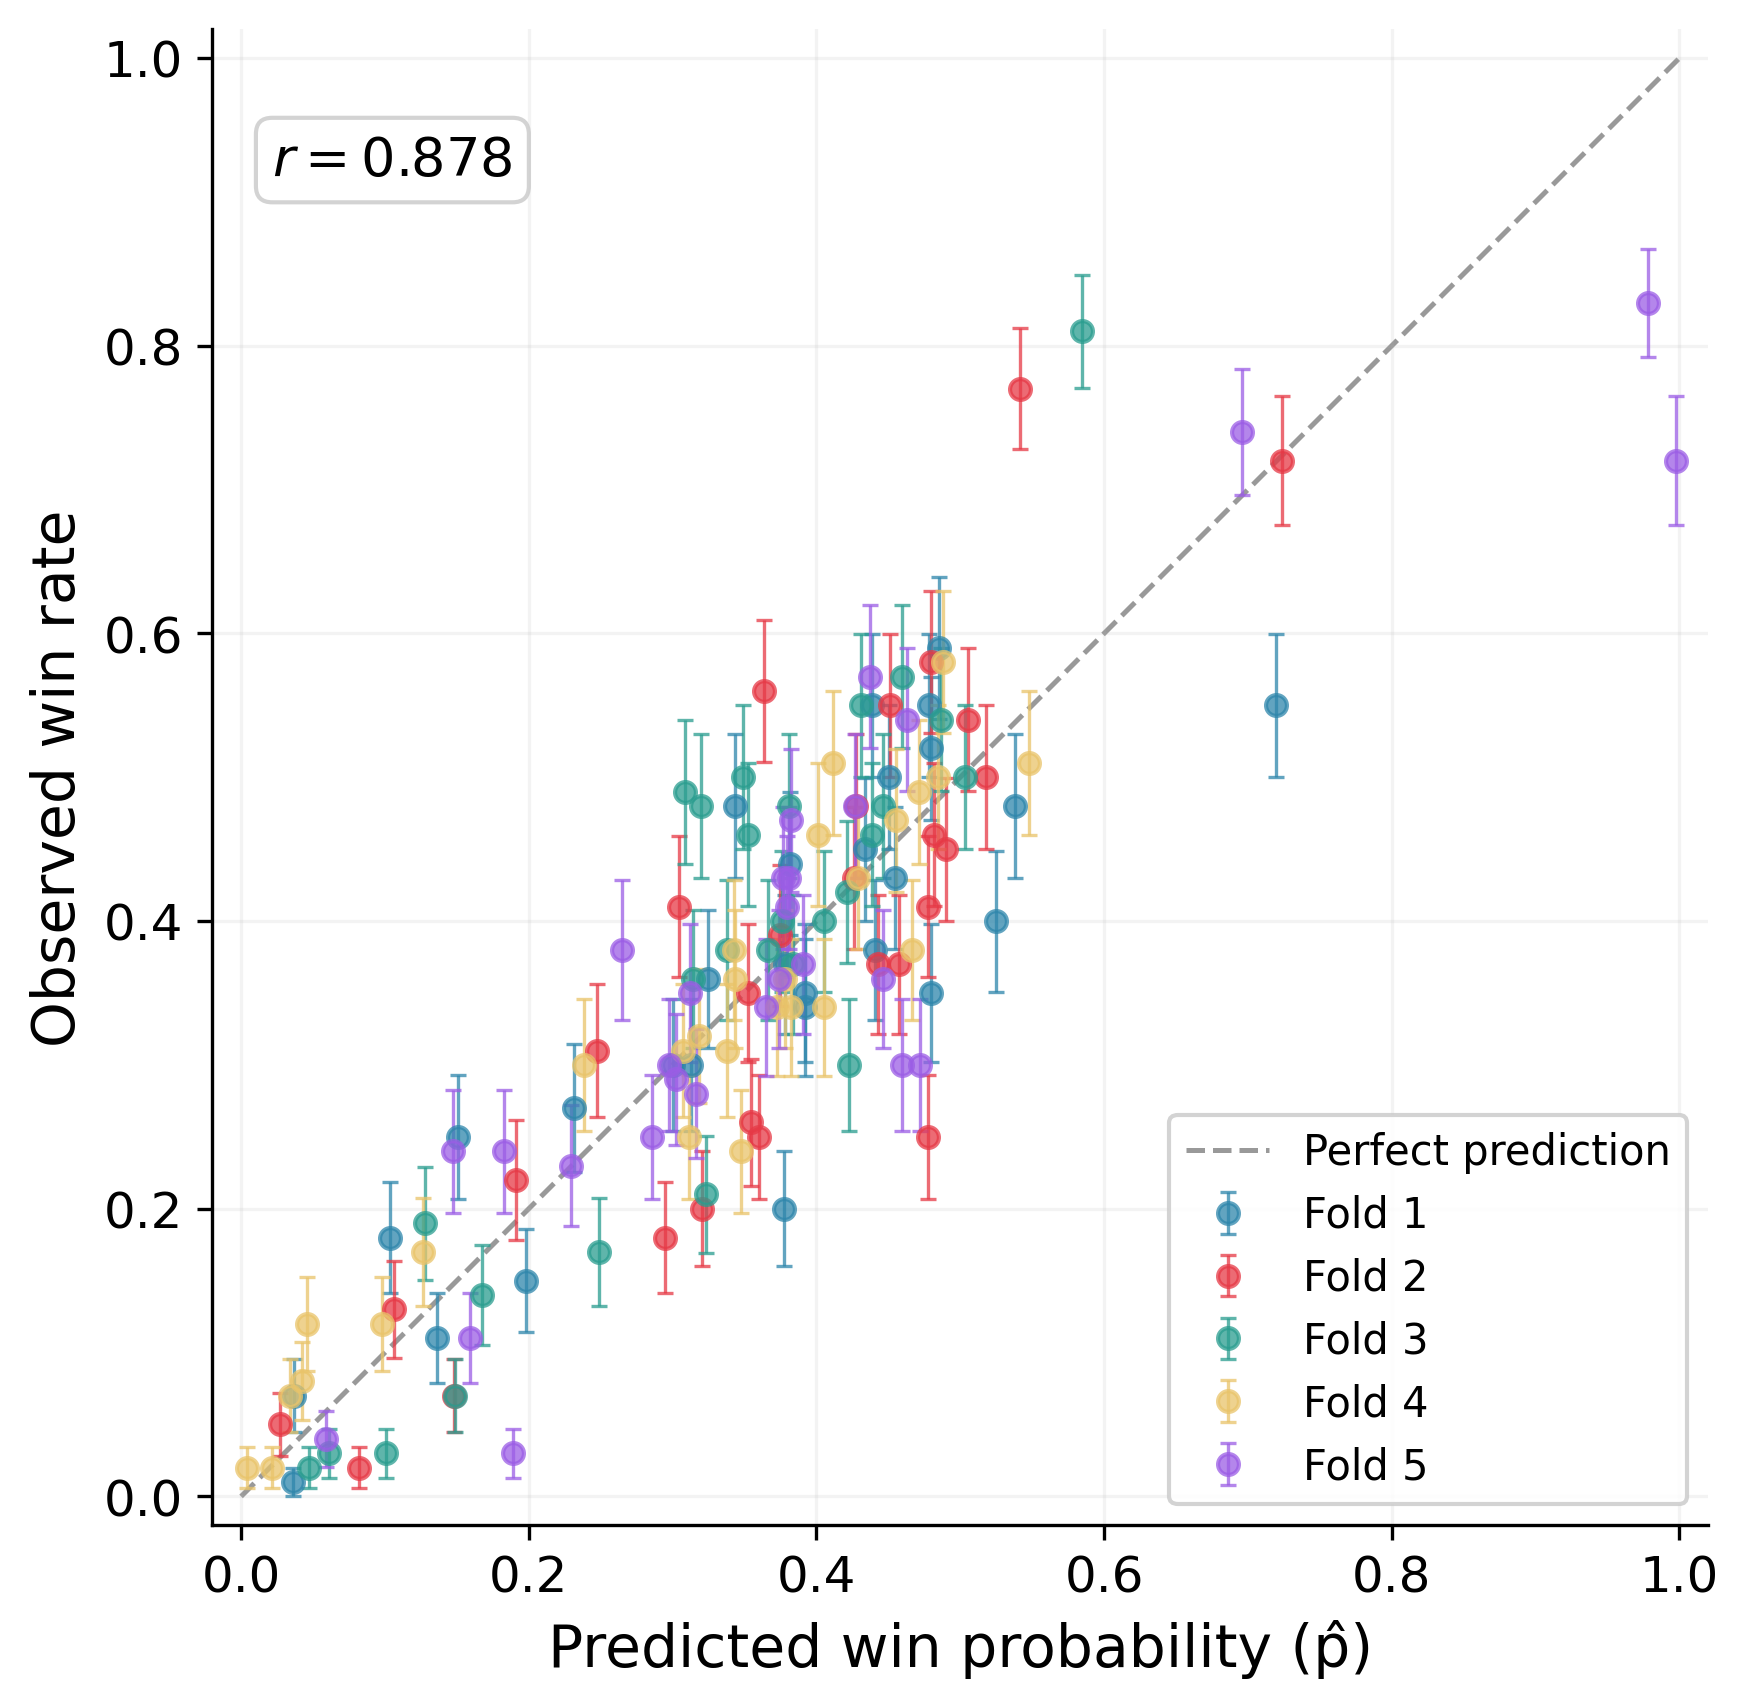
\includegraphics[height=0.72\textheight,keepaspectratio]{cv_scatter.png}\hspace{0.5em}%
    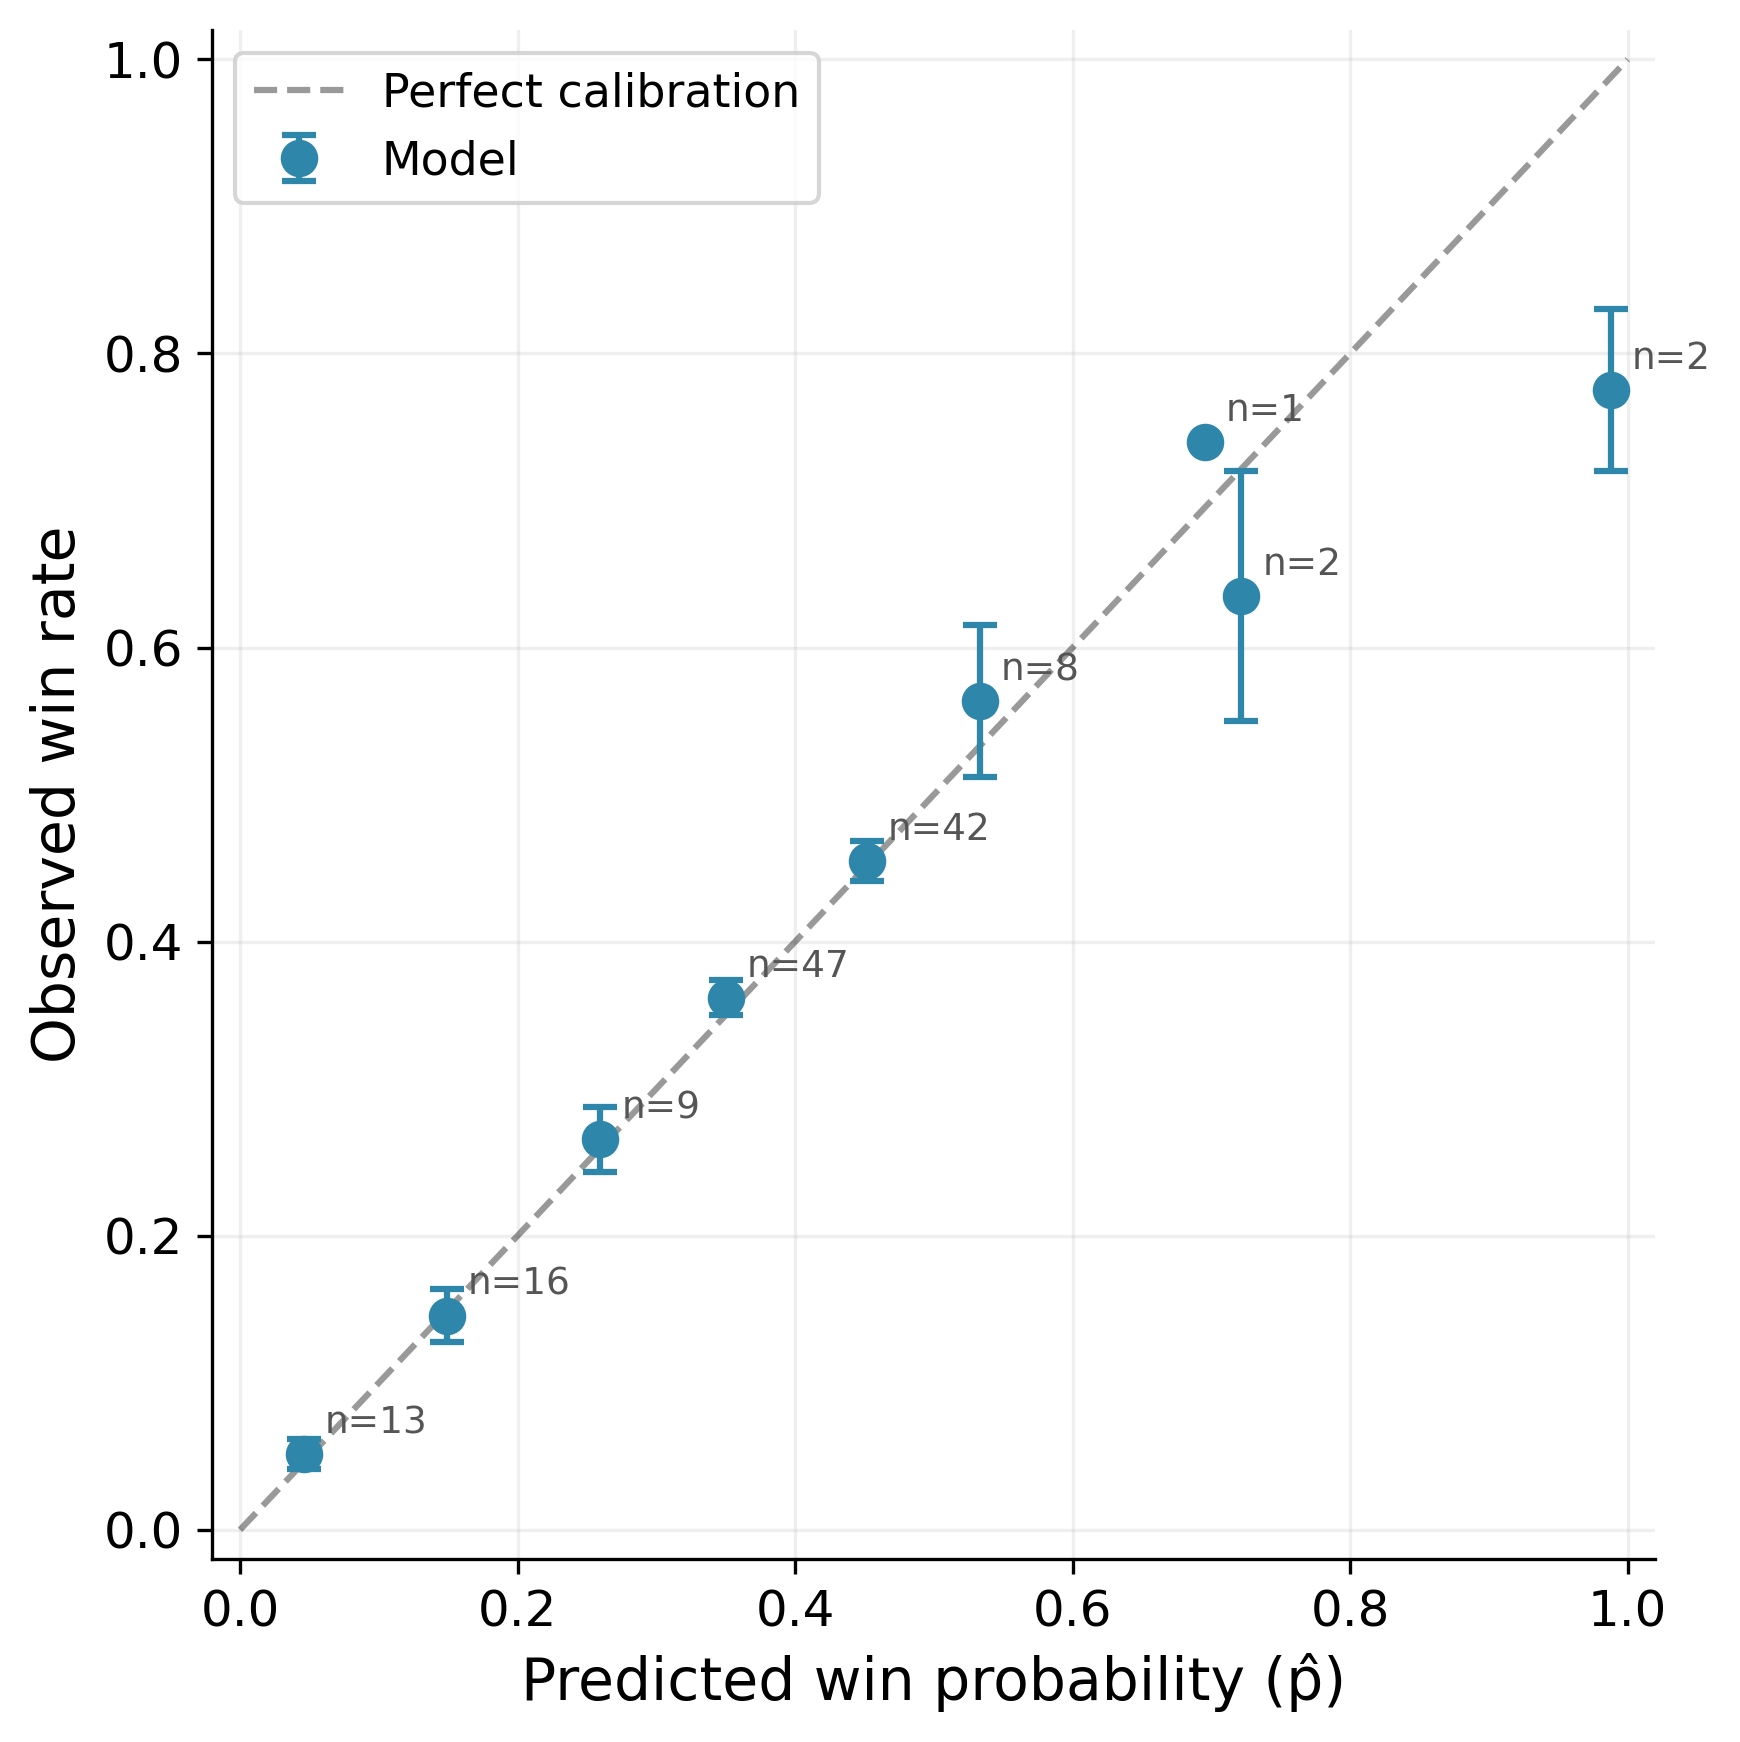
\includegraphics[height=0.72\textheight,keepaspectratio]{calibration_plot.png}
  \end{center}
  \vspace{0.1em}
  \centering
  {\small 5-fold cross-validation on 140 configurations: $76.6\%$ Brier-score reduction over baseline.}
\end{frame}

% ── Thank you ─────────────────────────────────────────────────────────────────
\begin{frame}[plain]
  \vfill\centering
  {\Large\bfseries Thank you}\\[1.2em]
  {\normalsize Davi Bastos Costa \quad Renato Vicente}\\[0.4em]
  {\small\color{black!50} TELUS Digital Research Hub \quad University of S\~{a}o Paulo}\\[1em]
  {\small\color{black!45} davi.costa@usp.br}\\[1.4em]
  \begin{tabular}{@{}c@{\hspace{2.8em}}c@{}}
    \qrcode[height=2.2cm]{https://github.com/bastoscostadavi/llm-mafia-game/tree/main/src} &
    \qrcode[height=2.2cm]{https://arxiv.org/abs/2509.23023} \\
    {\scriptsize\color{black!60} GitHub repo} &
    {\scriptsize\color{black!60} Paper}
  \end{tabular}
  \vfill
\end{frame}

% ── References ────────────────────────────────────────────────────────────────
\begin{frame}[allowframebreaks]{References}
  \bibliographystyle{unsrtnat}
  \bibliography{references}
\end{frame}

\end{document}
